%!TEX root = *.tex
%%%%%%%%%%%%%%%%%%
% カウンタのリセット
% 問題文
滑車と糸の質量は無視できるものとし,重力加速度を\g とする.

\begin{enumerate}[〔A〕]
  \setlength{\leftskip}{-1.5zw}
  \setlength{\itemindent}{1zw}\setlength{\labelsep}{0.5zw}
  \setlength{\labelwidth}{1zw}\setlength{\leftmargin}{1zw}
  \setlength{\itemsep}{0.5\baselineskip}
  \item 図1のように,なめらかに回る定滑車に伸縮しない糸をかけて,糸の一方に質量$m_1$のおもりA,他方に質量$m_2$のおもりBをつけて静かに放した.
  \begin{enumerate}[(1)]
    \setlength{\leftskip}{-2.5zw}
    \setlength{\itemindent}{1zw}\setlength{\labelsep}{1zw}
    \setlength{\labelwidth}{1zw}
    \item $m_1 > m_2$のとき,おもりAが下降する加速度の大きさを求めよ.
    \item 糸に働く張力の大きさを求めよ.
    \item $m_1 + m_2 = \text{一定}$として,糸の張力を最大にする$m_1$と$m_2$の関係を求めよ.
  \end{enumerate}
  \item 次に,図2のように定滑車の一方に質量$3M$のおもりCを,他方に動滑車をつり下げて,動滑車には質量$2M$のおもりDと質量$M$のおもりEをつり下げた.C,D,Eを同時に静かに放した.
  \begin{enumerate}[(1)]
    \setlength{\leftskip}{-2.5zw}
    \setlength{\itemindent}{1zw}\setlength{\labelsep}{1zw}
    \setlength{\labelwidth}{1zw}
    \setcounter{enumii}{3}
    \item おもりC,D,Eの加速度の大きさを求めよ.
    \item おもりD,E間の糸に働く張力の大きさを求めよ.
    \item おもりD,EはそのままでおもりCを$\C^\prime$に換えると,$\C^\prime$,D,Eを同時に静かに放しても,おもりは静止したまま動かなかった.
    このときのおもり$\C^\prime$の質量を求めよ.
  \end{enumerate}
\end{enumerate}

\begin{figure}[htbp]
  \centering
  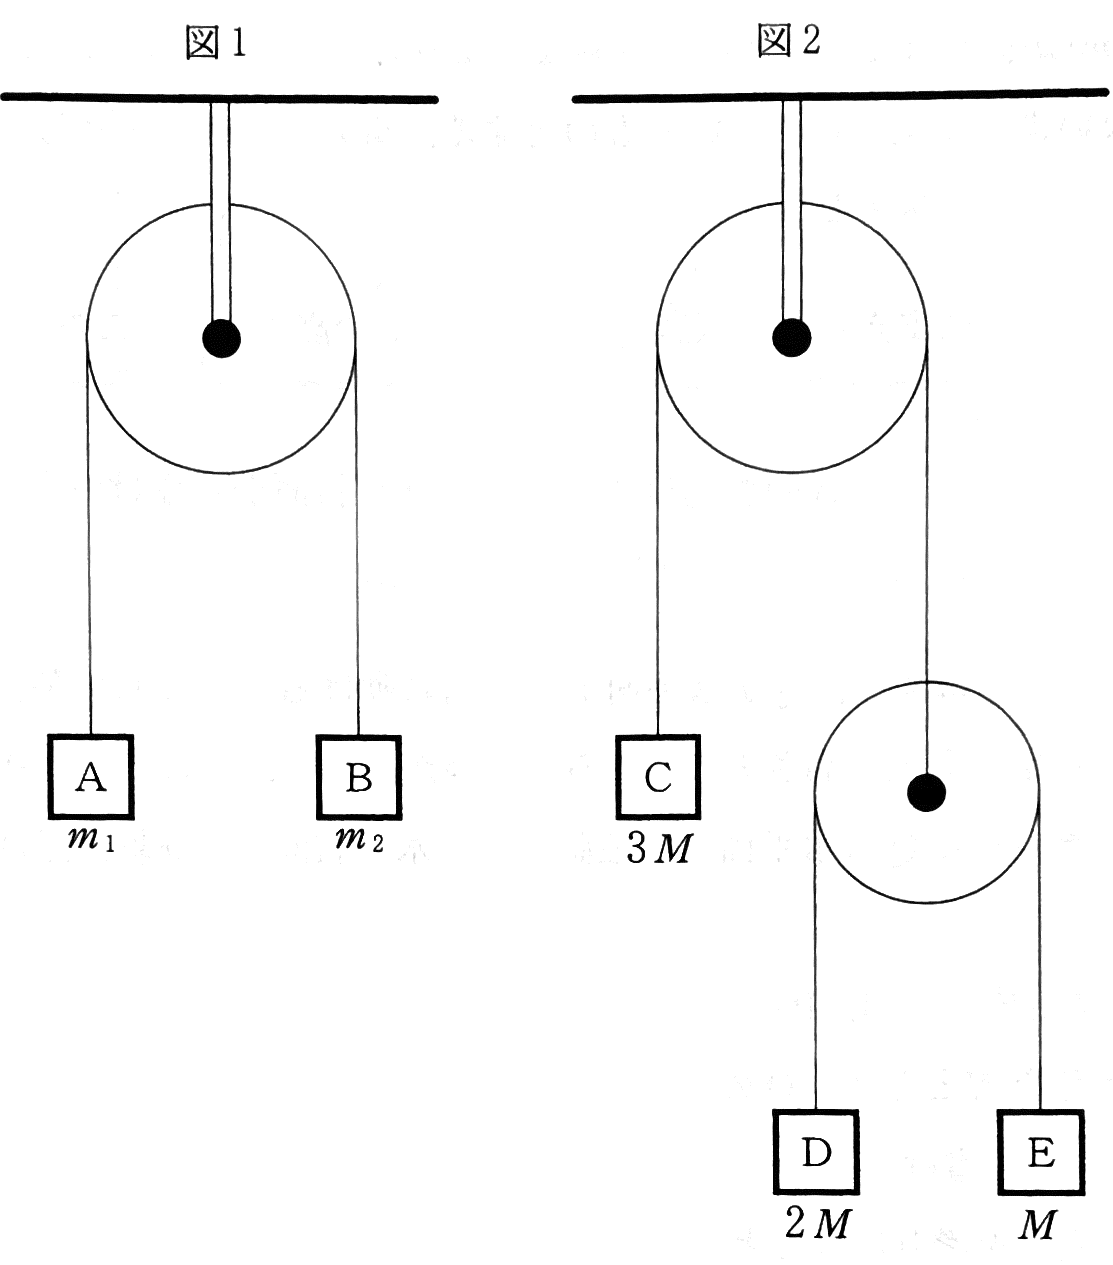
\includegraphics[width=20zw]{../graphs/se_1H_102.png}
\end{figure}


% メモ
\begin{comment}

\end{comment}


%%%%%%%%%%%%%%%%%%
